\iffalse
\let\negmedspace\undefined
\let\negthickspace\undefined
\documentclass[journal,12pt,twocolumn]{IEEEtran}
\usepackage{cite}
\usepackage{amsmath,amssymb,amsfonts}
\usepackage{graphicx}
\usepackage{textcomp}
\usepackage{xcolor}
\usepackage{txfonts}
\usepackage{listings}
\usepackage{enumitem}
\usepackage{mathtools}
\usepackage{gensymb}
\usepackage{comment}
\usepackage[breaklinks=true]{hyperref}
\usepackage{tkz-euclide} 
\usepackage{listings}
\usepackage{gvv}                                        
\def\inputGnumericTable{}                                 
\usepackage[latin1]{inputenc}                                
\usepackage{color}                                            
\usepackage{array}                                            
\usepackage{longtable}                                       
\usepackage{calc}                                             
\usepackage{multirow}                                         
\usepackage{hhline}                                           
\usepackage{ifthen}                                           
\usepackage{lscape}
\usepackage[export]{adjustbox}
\usepackage{pgfplots}
\newtheorem{theorem}{Theorem}[section]
\newtheorem{problem}{Problem}
\newtheorem{proposition}{Proposition}[section]
\newtheorem{lemma}{Lemma}[section]
\newtheorem{corollary}[theorem]{Corollary}
\newtheorem{example}{Example}[section]
\newtheorem{definition}[problem]{Definition}
\newcommand{\BEQA}{\begin{eqnarray}}
	\newcommand{\EEQA}{\end{eqnarray}}
\newcommand{\define}{\stackrel{\triangle}{=}}
\newtheorem{rem}{Remark}

\begin{document}
	\parindent 0px
	\bibliographystyle{IEEEtran}
	
	\vspace{3cm}
	
	\title{GATE:EE/63}
	\author{EE23BTECH11208 - Manohar K$^{*}$
	}
	\maketitle
	\newpage
	\bigskip
	
	% \renewcommand{\thefigure}{\theenumi}
	% \renewcommand{\thetable}{\theenumi}
	
	
	
	\textbf{Question:} \hspace{2pt} A signal $x\brak{t}=2\cos{(180\pi t)}\cos{(60\pi t)}$ is sampled at 200 Hz and then passed through an ideal low pass filter having cut-off frequency of 100 Hz.\\
	The maximum Frequency present in the filtered  signal in Hz is \rule{1cm}{0.5mm} (Round off to the nearest integer.) \hfill (GATE 2023 EE)\\
	\noindent \textbf{Solution:}\\
\fi
	\begin{figure}[ht]
		\centering
		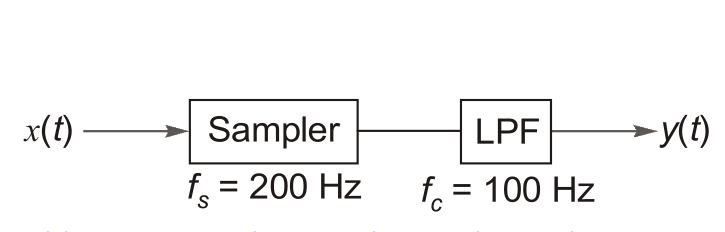
\includegraphics[width=1\linewidth]{2023/EE/63/figs/answerdia.png}
	\end{figure}
	Given, \\
	
	\begin{align}
		x\brak{t}&=\cos\brak{240\pi t} + \cos\brak{120\pi t}
	\end{align}\\
	\begin{table}[h]
		\centering
		
\begin{tabular}{|c|c|c|}
	\hline
	\textbf{symbol} & \textbf{value} & \textbf{description} \\
	\hline
	$x(t)$ & $2\cos{(180\pi t)}\cos{(60\pi t)}$ & input signal \\
	\hline
	$f_s$ & $200Hz$ & sampling frequency \\
	\hline
	$f_c$ & $100Hz$ & cut-off frequency \\
	\hline
	$y(t)$ &  & output signal \\
	\hline
	$f_1$ & $120Hz$ & first signal frequency \\
	\hline
	$f_2$ & $60Hz$ & second signal frequency \\
	\hline
\end{tabular}

		\caption{Parameters}
		\label{tab:GATE.EE.2023.63}
	\end{table}\\
	Aliased frequencies when $f_1$ frequency signal is sampled at $200Hz$\\
	\begin{align}
		& f_1 , \abs{f_s\pm f_1} , \abs{2f_s \pm f_1} \dots\\
		& 120, 80,340,280,520 \dots
	\end{align}
	Aliased frequencies when $f_2$ frequency signal is sampled at $200Hz$\\
	\begin{align}
		& f_2 , \abs{f_s\pm f_2} , \abs{2f_s\pm f_2} \dots\\
		& 60 , 140,260,340,460 \dots 
	\end{align}
\begin{figure}
	\centering
	\begin{tikzpicture}
\begin{axis}[
    axis lines=middle,
    xlabel=$f$,
    ylabel=$X(f)$,
    ymax=1,
    ymin=0,
    xmin=-240,
    xmax=240,
    xtick={ -120, -60, 60, 120},
    ytick={0,1},
    yticklabels={0,1},
    ticklabel style={font=\tiny},
    enlargelimits={abs=0.2},
    clip=false
]
% One-sided arrows
\draw[->, >=latex, blue, thick] (axis cs: -120, 0) -- (axis cs: -120, 1);
\draw[->, >=latex, blue, thick] (axis cs: -60, 0) -- (axis cs: -60, 1);
\draw[->, >=latex, blue, thick] (axis cs: 60, 0) -- (axis cs: 60, 1);
\draw[->, >=latex, blue, thick] (axis cs: 120, 0) -- (axis cs: 120, 1);
\end{axis}
\end{tikzpicture}

	\caption{delta function of input signal }
\end{figure}\\
	
	
\begin{figure}
	\centering
	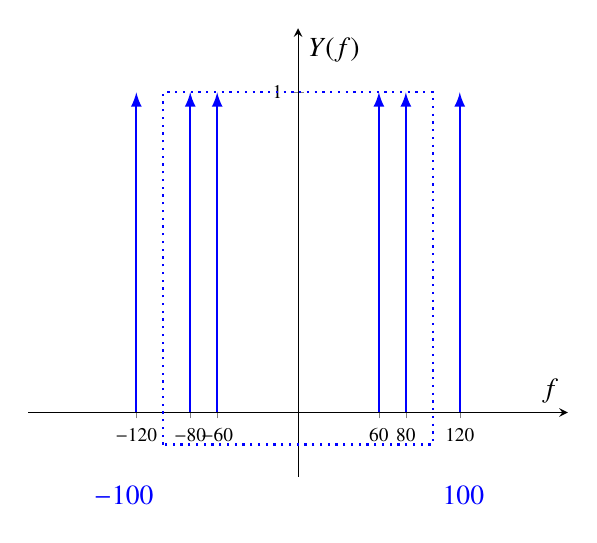
\begin{tikzpicture}
\begin{axis}[
    axis lines=middle,
    xlabel=$f$,
    ylabel=$Y(f)$,
    ymax=1,
    ymin=0,
    xmin=-200,
    xmax=200,
    xtick={ -120, -80, -60, 60, 80, 120},
    ytick={0,1},
    yticklabels={0,1},
    ticklabel style={font=\scriptsize},
    enlargelimits={abs=0.2},
    clip=false
]
% One-sided arrows
\draw[->, >=latex, blue, thick] (axis cs: -120, 0) -- (axis cs: -120, 1);
\draw[->, >=latex, blue, thick] (axis cs: -80, 0) -- (axis cs: -80, 1);
\draw[->, >=latex, blue, thick] (axis cs: -60, 0) -- (axis cs: -60, 1);
\draw[->, >=latex, blue, thick] (axis cs: 60, 0) -- (axis cs: 60, 1);
\draw[->, >=latex, blue, thick] (axis cs: 80, 0) -- (axis cs: 80, 1);
\draw[->, >=latex, blue, thick] (axis cs: 120, 0) -- (axis cs: 120, 1);
% Dotted box
\draw[blue, dotted, thick] (axis cs: -100, -0.1) rectangle (axis cs: 100, 1);
\node[blue, below right] at (axis cs: 100, -0.2) {$100$};
\node[blue, below left] at (axis cs: -100, -0.2) {$-100$};
\end{axis}
\end{tikzpicture}

	\caption{delta function of sampled and filtered signal }
\end{figure}
	from table $f_c = 100Hz$ \\
	LPF output : $60Hz$ , $80Hz$\\
	Maximum Frequency present in the filtered signal is $80Hz$.
	
	
	
